\section{Introduction}

Travelling salesman problem requires to find the shortest path visiting all the nodes in a graph just once. The \textit{TSP} is an NP-hard problem, namely a problem that cannot be solved in polynomial time, however during past decades many heuristics and algorithms were invented to find an approximate solution of the problem. One of them, used in the project, is a genetic algorithms approach that mimics the genetic evolution of species. 

A genetic algorithm starts with a set of chromosomes (\textit{population}) that are typically randomly defined. Then these chromosomes are evaluated and a reproductive opportunity is allocated for each of them in such a way that those chromosomes which represent a better solution to the target problems are given more chance to ``reproduce'' than those chromosomes which are poorer solution \cite{genetic-algorithm-tutorial}. After the selection phase the crossover and mutations operations are applied to produce a new population for the next generation. It is helpful to view an entire generation phase as a two stage process, it starts with a population that after the selection phase becomes an intermediate population. Then the new population is produced by applying recombination operations, according to probability, on the intermediate population. 

In the project \textit{TSP} was modelled as an \textit{undirected weighted graph}, a chromosome represents a route that visits each city and returns to the origin city and our goal was to find a good chromosome that minimizes the length of this complete route on the graph. For each chromosome the evaluation function, that provides the performance, was the sum of all the edges length inside it. To verify the correctness of the algorithm for each version developed, the generation number with the current generation best chromosome path value were saved and then plotted. This was done for five thousand generations with chromosomes of length equal to two hundred. As we can see from the plots obtained (figure  \ref{algorithmsConvergence}) for every version developed the convergence of the algorithm to a lower route on the graph was obtained. 
\vspace{0.6em}

\begin{figure}[H]
	\minipage{0.32\textwidth}%
	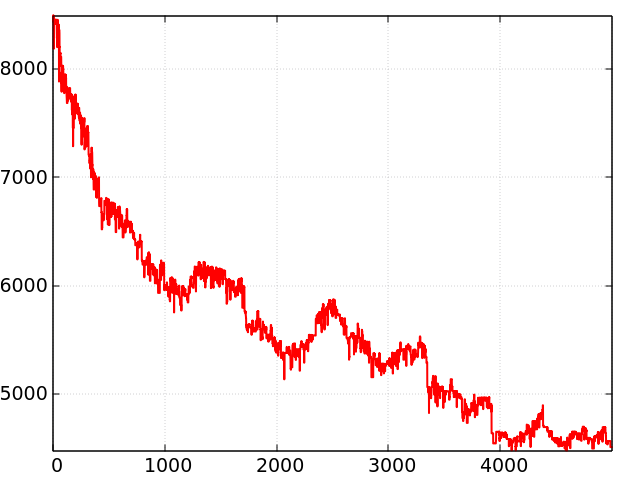
\includegraphics[width=\linewidth]{benchmark/convergence/sequentialConvergence.png}
	\subcaption{Sequential}\label{fig:sequential_convergence}
	\endminipage\hfill
	\minipage{0.32\textwidth}%
	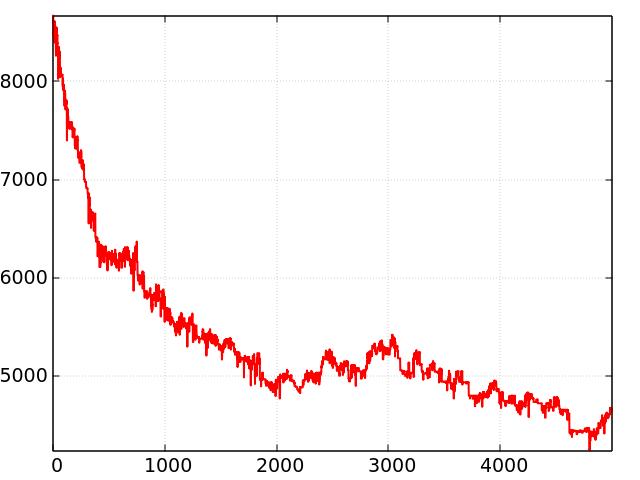
\includegraphics[width=\linewidth]{benchmark/convergence/standardConvergence.png}
	\subcaption{Standard thread}\label{fig:standard_convergence}
	\endminipage\hfill
	\minipage{0.32\textwidth}%
	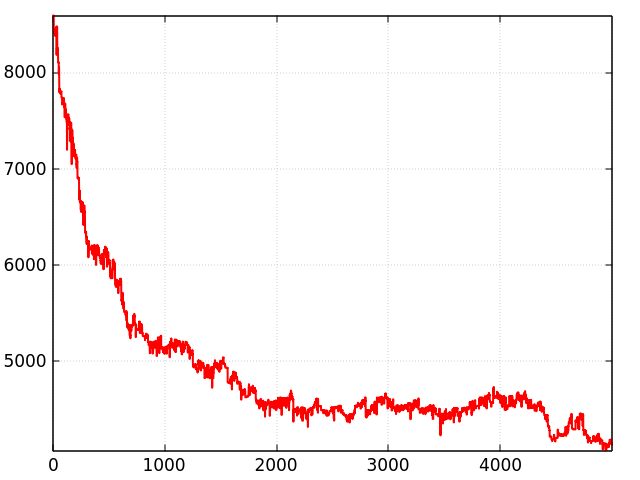
\includegraphics[width=\linewidth]{benchmark/convergence/fastflowConvergence.png}
	\subcaption{Fastflow}\label{fig:fastflow_convergence}
	\endminipage
	\caption{}\label{algorithmsConvergence}
\end{figure}

\subsection{Measures}
To compare and model the performance of a parallel program two performance indicators were used, \textit{speedup} and \textit{scalability}. For these metrics the speedup asymptote is given by $f(n) = n$.
\subsubsection{Speedup}
The \textit{speedup} is the ratio between the best known sequential execution time and the parallel execution time. It gives a measure of how good is our parallelization with respect to the best sequential computation. It is a function of \textit{n} the parallelism degree of the parallel execution.
\begin{equation}
speedup(n) = \frac{T_{seq}}{T_{par}(n)}
\end{equation} 
\vspace{-2em}
\subsubsection{Scalability}
The \textit{scalability} is the ratio between the parallel execution with degree equal to 1 and the parallel execution time with parallelism degree equal to \textit{n}. It measures how efficient is the parallel implementation in obtaining better performance on bigger parallelism degree.
\begin{equation}
scalab(n) = \frac{T_{par}(1)}{T_{par}(n)}
\end{equation}

